Để tạo mô phỏng các máy tính trong mạng tôi sử dụng 3 máy ảo với phần mềm Virtualbox.

Mạng mô phỏng được biểu diễn như trong hình \ref{fig:network-model}.

\begin{figure}[ht!]
	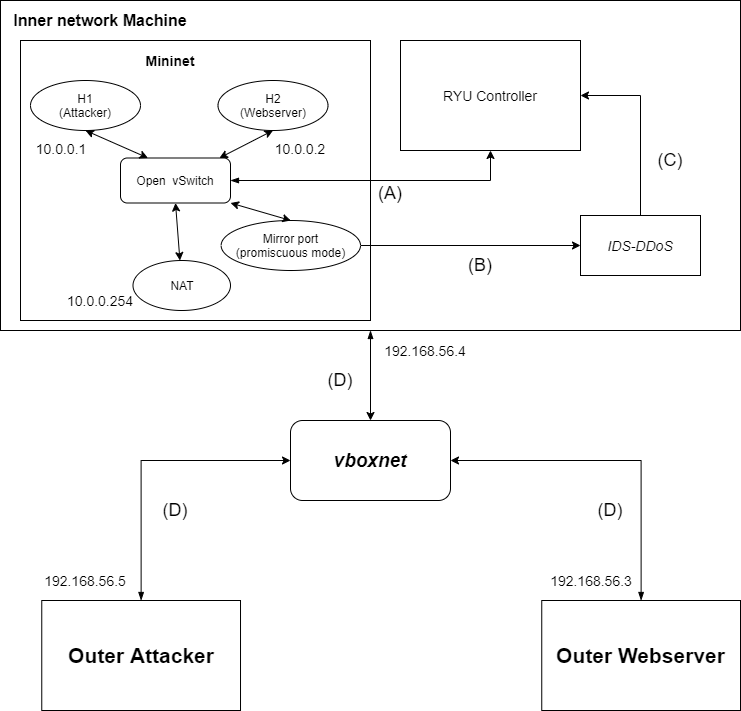
\includegraphics[width=\linewidth]{fig/network-model.png}
	\caption{Mạng mô phỏng}
	\label{fig:network-model}
\end{figure}

Các máy ảo trong mạng sẽ gồm Inner Network Machine, Outer Attacker và Outter Webserver. Các máy này được nối với nhau qua 1 mạng ảo Host-only (D) của Virtualbox với địa chỉ đường mạng là 192.168.56.0. Thông tin về các máy này được ghi trong bảng \ref{tab:host-description}.

\begin{table}[ht!]
	\begin{tabular}{|l|l|l|l|}
		\hline
		\multicolumn{1}{|c|}{\textbf{Máy}} &
		\multicolumn{1}{c|}{\textbf{Vai trò}} &
		\multicolumn{1}{c|}{\textbf{Địa chỉ IP}} &
		\multicolumn{1}{c|}{\textbf{Cấu hình}} \\ \hline
		Inner Network Machine &
		\begin{tabular}[c]{@{}l@{}}Chứa   mạng ảo \\ SDN được tạo \\ bằng Mininet, \\ RYU SDN \\ Controller và phần \\ mềm IDS-DDoS.\end{tabular} &
		192.168.56.4 &
		\begin{tabular}[c]{@{}l@{}}HĐH Ubuntu \\ 18.04 64bit\\ CPU 6 threads\\ RAM 4GB\end{tabular} \\ \hline
		Outer Webserver &
		\begin{tabular}[c]{@{}l@{}}Chứa   một trang \\ web tĩnh tạo vởi\\ SimpleHTTP \\ python\end{tabular} &
		192.168.56.3 &
		\begin{tabular}[c]{@{}l@{}}HĐH Ubuntu \\ server 18.04   32bit\\ CPU 1 thread\\ RAM 1GB\end{tabular} \\ \hline
		Outer Attacker &
		\begin{tabular}[c]{@{}l@{}}Dùng   để chạy\\ công cụ tấn công\\ DDoS Hoic\end{tabular} &
		192.168.56.5 &
		\begin{tabular}[c]{@{}l@{}}HĐH Windows 7 \\ 32bit\\ CPU 2 threads\\ RAM 2GB\end{tabular} \\ \hline
	\end{tabular}
\caption{Mô tả các máy tính trong mạng}
\label{tab:host-description}
\end{table}

\textit{Inner network Machine}

\begin{itemize}
	\item [--] Mạng SDN được kết nối 2 chiều với RYU Controller thông qua TCP localhost (A).
	\item [--] Mirror port là 1 card mạng ảo ở chế độ promiscious dùng để chuyển tất cả traffic từ H1 và H2 vào đây. Card mạng này được phần mềm IDS-DDoS lắng nghe để bắt các gói tin và phân loại luồng (B).
	\item [--] RYU Controller và phần mềm IDS-DDoS giao tiếp với nhau thông qua unixsocket (C).
\end{itemize}

\textit{Mạng SDN}

\begin{itemize}
	\item [--] H1, H2 là các host trong mạng SDN. Trong đó H1 dùng để chạy phần mềm tấn công DDoS Hulk, H1 dùng để làm 1 webserver. 
	\item [--] Để H1, H2 có thể giao tiếp với bên ngoài, Open vSwitch được trang bị thêm 1 thiết bị NAT.
	\item [--] Ngược lại, để máy bên ngoài có thể giao tiếp với Webserver H2, các lệnh ''iptables nat'' được dùng sao cho tất cả gói tin đi tới  port 80 của máy  Inner network machine sẽ được chuyển vào port 80 của thiết bị NAT trong SDN, từ đó, tất cả các gói tin đi vào port 80 sẽ được chuyển vào port 80 của máy H2. Mô hình như hình \ref{fig:nat}.
\end{itemize}

\begin{figure}[ht!]
	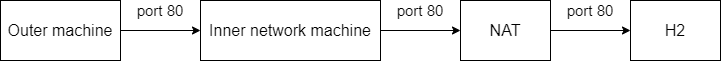
\includegraphics[width=\linewidth]{fig/nat.png}
	\caption{Mô hình NAT port}
	\label{fig:nat}
\end{figure}